\documentclass[a4paper,12pt,oneside]{article}
\usepackage{amsmath}
\usepackage{mathtools}
% \usepackage{caption}
\usepackage[labelformat=empty]{caption}
\usepackage{mathptmx}
\usepackage{fixltx2e}
\usepackage{graphicx}
\usepackage[margin=1.0in]{geometry}
\usepackage{float}
\let\counterwithout\relax
\let\counterwithin\relax
\usepackage{setspace}
\usepackage{chngcntr}
\usepackage{fancyhdr}
\usepackage{etoolbox}
\patchcmd{\thebibliography}{\section*{\refname}}{}{}{}


\pagestyle{fancy}
\fancyhf{}
\rfoot{\thepage}
%\renewcommand{\headrulewidth}{0.0pt}
%\renewcommand{\footrulewidth}{0.0pt}


\begin{document}
\thispagestyle{empty}
%\pagenumbering{gobble}
\begin{center}

\large{\textbf{{A Smart Home Energy Management System
Using IoT and Big Data Analytics Approach}}}
\setlength{\baselineskip}{1.5\baselineskip}
\\
\vspace{5mm}
\textbf{SEMINAR REPORT}

Submitted in the partial fulfilment of the award of the degree
of
\\
\textbf{Bachelor of Technology}
\\
in
\\
\textbf{Computer Science \& Engineering}
\\
of
\\
\textbf{APJ Abdul Kalam Technological University}
\\
by
\\
\textbf{S HEMANTH}
\\
\vspace{5mm}
\begin{figure}[H]
\centering

\includegraphics[scale=0.5]{ceclogo.png}
\end{figure}
\textbf{November 2019}
\vspace{8mm}
\\
Department of Computer Engineering
\\
College of Engineering, Chengannur, Kerala -689121
\\
Phone: (0479) 2454125, 2451424; Fax: (0479) 2451424
\\
\end{center}

\newpage
\thispagestyle{empty}
\begin{center}
\setlength{\baselineskip}{1.5\baselineskip}
{\large\textbf{COLLEGE OF ENGINEERING, CHENGANNUR}}
\\
{\large\textbf{KERALA}}
\\
\begin{figure}[H]
\centering

\includegraphics[scale=0.5]{ceclogo.png}
\end{figure}
\setlength{\baselineskip}{1.5\baselineskip}
\textbf{Department of Computer Engineering}
\\
\textbf{CERTIFICATE}
\\
This is to certify that the seminar entitled
\\
\textbf{A Smart Home Energy Management System
Using IoT and Big Data Analytics Approach}
\\
Submitted by
\\
\textbf{S HEMANTH}
\\
is a bonafide record of the work done by him.
\end{center}
\vspace{30ex}
%\textbf{Mrs.Sheeba}
\hspace{55ex}
%\textbf{Dr. Smitha Dharan}
\\

\hspace{0ex}
\textbf{Co-ordinator}
\hspace{18ex}
\textbf{Guide}
\hspace{18ex}
\textbf{Head of the Department}
\newpage
\pagenumbering{roman}
\renewcommand{\headrulewidth}{0.0pt}
\renewcommand{\footrulewidth}{0.0pt}
\begin{center}
\large{\textbf{ACKNOWLEDGEMENT}}
\end{center}
\vspace{6ex}
\setlength{\baselineskip}{1.5\baselineskip}
\paragraph{}
I am greatly indebted to \textbf{God Almighty} for being the guiding light throughout with his
abundant grace and blessings that strengthened me to do this endeavour with confidence.
\paragraph{}
I express my heartfelt gratitude towards \textbf{Dr. Jacob Thomas V.}, Principal, College
of Engineering Chengannur for extending all the facilities required for doing my seminar.
I would also like to thank \textbf{Dr. Smitha Dharan}, Head, Department of Computer
Engineering, for providing constant support and encouragement.
\paragraph{}
Now I extend my sincere thanks to my seminar co-ordinators \textbf{Mrs. Shiny B}, Assistant
Professor in Computer Engineering for guiding me in my work and providing timely
advices and valuable suggestions.
\paragraph{}
Last but not the least, I extend my heartfelt gratitude to my parents and friends for
their support and assistance.	
\pagenumbering{gobble}

\newpage
\begin{center}
\large{\textbf{ABSTRACT}}
\end{center}
\vspace{4ex}
\paragraph{}
Increasing cost and demand of energy has led many
organizations to find smart ways for monitoring, controlling and
saving energy. A smart Energy Management System (EMS) can
contribute towards cutting the costs while still meeting energy
demand. The emerging technologies of Internet of Things (IoT)
and Big Data can be utilized to better manage energy
consumption in residential, commercial, and industrial sectors.
\paragraph{}
This report presents an Energy Management System (EMS) for
smart homes. In this system, each home device is interfaced with
a data acquisition module that is an IoT object with a unique IP
address resulting in a large mesh wireless network of devices.
The data acquisition System on Chip (SoC) module collects
energy consumption data from each device of each smart home
and transmits the data to a centralized server for further
processing and analysis. This information from all residential
areas accumulates in the utility’s server as Big Data. The
proposed EMS utilizes off-the-shelf Business Intelligence (BI) and
Big Data analytics software packages to better manage energy
consumption and to meet consumer demand.
\setlength{\baselineskip}{1.0\baselineskip}

% Table of content Page
\newpage
\begin{center}
\tableofcontents
\end{center}



% List of Figures Page
\newpage
\thispagestyle{plain}
\begin{center}
\listoffigures
\end{center}



\newpage
\rfoot{\thepage}
\lhead{\textit{A Smart Home Energy Management System
Using IoT and Big Data Analytics Approach}}
\lfoot{\textit{College of Engineering Chengannur}}
\rfoot{\thepage}
\renewcommand{\headrulewidth}{0.0pt}
\renewcommand{\footrulewidth}{0.0pt}
\renewcommand{\headrulewidth}{0.0pt}
\renewcommand{\footrulewidth}{0.0pt}
\section{INTRODUCTION}
\pagenumbering{arabic}
\paragraph{}
Effective management of Energy consumption in smart homes saves money,
enhances sustainability and reduces carbon footprint at
large. However, the lack of low cost, easy to deploy, and low
maintenance technology has somewhat limited a large-scale deployment of such systems.
\paragraph{}
The sheer quantity of data
collected throughout different cities of a country presents
multiple challenges in data storage, organization, and analysis.
Internet of Things (IoT) technology and Big Data are natural
candidates to address these challenges. IoT technologies can
provide a ubiquitous computing platform to sense, monitor
and control the household appliances energy consumption on a
large scale. This data is collected using many different
wireless sensors installed in residential units. Similarly, Big
Data technology can be utilized to collect and analyze large
amounts of data [1]. Data analytics on this data using business
intelligence (BI) platform [2] plays an essential role in energy
management decisions for homeowners and the utility alike.
The data can be monitored, collected and analyzed using
predictive analysis and advanced methods to actionable
information in the form of reports, graphs and charts. Thus,
this analyzed data in real-time can aid home owners, utilities
and utility eco-systems providers to gain significant insights
on energy consumption of smart homes. The energy service
providers can use the power consumption data available with
analytics engine to provide flexible and on-demand supply
with appropriate energy marketing strategies. The consumers,
being aware of their consumption behavior and having a close
interaction with the electricity utilities, can adjust and
optimize their power consumption and reduce their electricity
bills.
\paragraph{}
Finally, as
an additional advantage, the use of IoT also enables seamless
remote access control of home devices where the customers
get online access to the ON/OFF usage pattern of in home
appliances via a personal computer or a mobile phone.
\paragraph{}
Rest of the report is organized as follows. Previous work in
using Home Energy management System (HEMS) is
presented next. This is followed by the proposed system
requirements. The system architecture is presented next
followed by a description of implementation details.
Evaluation and testing is described and succeeded by the
conclusion.

\newpage
\section{RELATED WORK}
\subsection{Home Energy Management System (HEMS) using a ZigBee Module}
\paragraph{}
In [3, 4, 5], an
implementation of a HEMS Unit in a Wireless Sensor
Network using a ZigBee Module to communicate with sensor
nodes, is presented. The system monitors the device
consumption data and sends control signals to end nodes
during peak load hours. However, the lifetime of a WSN
network deteriorates with time due to the deployment of new
sensors in the network. Additionally, Han et al. in [6]
introduced a system for monitoring power consumption using
ZigBee as the communication protocol in a WSN. However,
in this system the data was collected and aggregated solely by
the home server which could lead to data loss in case of a
system failure. Moreover, a bridge between ZigBee and
TCP/IP stack would be required to connect this system to a
community of homes.

\subsection{Extending the Previous Work}
In [7, 8], the above mentioned WSN networks have been extended
to wider ranges in the IoT paradigm utilizing the GSM/GPRS
networks to remotely control the end-devices.

\subsection{An Integrated Cloud-based Smart Home Management System}
In this paper [12], a hierarchical, smart-home service architecture employed with
multiple in-home displays for user interfaces is described by them.
In this research, a home controller system interfaced
with device sensors is responsible for aggregated energy
reporting of all devices to home owners. For community
representatives, a community broker server is integrated with
different home network devices such as security cameras
within a community. Furthermore, a comparative analysis
between Message Queuing Telemetry Transport Protocol
(MQTT) and Hypertext Transfer Protocol (HTTP) is also
performed to determine which protocol was more efficient in
providing home control services [12]. The design of the
proposed architecture, however, lacks the incorporation of Big
Data which is instrumental in processing and analyzing huge
volume of data collected from several home sensor networks.

\newpage
\subsection{Developments of the in-home Display Systems for Residential Energy Monitoring}
Multiple in-home display systems (IHDs) and automatic
meter reading systems (AMR) were discussed in the context of
providing energy management information in [14]. Depending
on the ambient conditions, the smart home systems could
choose the display devices such as TV, smartphone or tablet
computers and accordingly select the appropriate user
interface. The architecture, however, lacked a standardized
user interface for all the home devices that could accomplish
the requirement for multiple displays.

\subsection{Home energy management system based on power line communication}
This architecture of HEMS utilizing power line communication was addressed
in [15]. Using smart meter data, this HEMS can monitor and provide real-time information on home energy consumption
along with online access to devices status, thus allowing
remote control of devices by customers. The proposed design
is based on standard HTTP protocol and does not provide
support for lighter-weight communication protocol like
MQTT which is essential to scale up the system in order to
accommodate multiple residential areas.



\newpage
\section{PROPOSED SYSTEM REQUIREMENTS}
The functional requirements of the system are specified as
general functional requirements and specific system
requirements. The general requirements are the system’s
functionality and specific requirements are different business
processes delivered. Non-functional requirements comprise of
system’s attributes such as scalability, security, privacy.
\paragraph{}
The proposed system’s functional requirements are:
\begin{itemize}
    \item The SoC should gather power consumption information
    and the ambient condition information periodically, and
    send it to a centralized server.
    \item The server should parse the information and transmit
    the readings to a central data storage system or
    database.
    \item The stored data should be used by analytics engine to
    process it and generate reports, graphs, and charts.
    \item Clients should be able to view the generated graphs
    through a cross-platform mobile application.
    \item Depending on the user privileges, the application
    should render different services to each user such as
    viewing reports, device status, and remote control of
    device or bill payment.
\end{itemize}
\newpage
\paragraph{}
The proposed system’s non-functional requirements are:
\begin{itemize}
    \item Scalability
    \paragraph{}The data is collected and analyzed on a national level
    accommodating four different levels of stakeholders: Home
    Owner, Community Representative, State Representative
    and Country Representative. Each stakeholder has
    its respective view of the data and services offered. The
    six business processes mentioned above should be applied
    to each stakeholder as required. To serve these levels of
    clients, the system should be based on an easily scalable
    architecture.
    \item Security
    \paragraph{}Security of the system is important as a minor flaw in
    system design can lead to catastrophic disasters. Multiple
    levels of security such as secured web service calls using https
    must be implemented to ensure protected communication of
    the system.
    \item Privacy
    \paragraph{}
    The communication between server and end devices should
    be private. Access control using two factor authentication and
    proper encryption techniques should be utilized to prevent
    illegitimate users from prying over the data.
    
\end{itemize}

\newpage
\section{SYSTEM ARCHITECTURE}
Based on the above system requirements, the proposed
system’s hardware and software architecture are as follows:

\begin{figure}[H]
\includegraphics[height=5cm,width=10cm]{figure1.png}
%\counterwithin{figure}{section}
\centering
\caption{\textbf{Figure 1.} Systerm Architecture}
\end{figure}

\subsection{Hardware Architecture}
\subsubsection{Sensors and Actuators}
As the proposed system is to monitor and control the AC
units, an integrated temperature and humidity sensor is
interfaced with the microcontroller to measure the ambient
conditions. In addition, a solid state relay is controlled by the microcontroller
to switch ON/OFF the devices accordingly. A
current sensor is used to measure the AC current to calculate
the power consumption.
\subsubsection{High-end Microcontroller}
A SoC high end microcontroller is used as edge device data
acquisition module that manages the HVAC unit. The
compact sized, high speed and lightweight SoC is suitable for
residential areas. Table I displays the specifications of the
micro-controller used in this study.
\subsubsection{Servers}
In the proposed architecture, the servers are high-end PCs
which can also be deployed on Cloud for wide-scale
accessibility. The installed servers are: MQTT Broker, highly
scalable Storage Server, Analytics Engine server, and a Web
server. The functionality of each server developed and utilized
will be explained in the software architecture section.

\begin{figure}[H]
\includegraphics{figure2.png}
%\counterwithin{figure}{section}
\centering
\caption{\textbf{Table 1.} MICRO-CONTROLLER SPECIFICATION}
\end{figure}

\subsection{Research Materials}
\paragraph{}
A writing task and a survey questionnaire were developed to evaluate whether learners benefitted from the proposed system. The purpose of this study is to investigate learners’ general performance in emotion word use. Thus, Ekman’s six emotion categories was adopted, the most used characterization in many previous studies, while designing the writing task. For each category, we designed three individual scenarios, which were determined based on the results of a pilot study. The scenarios, described in the participants’ first language to avoid misunderstandings, were to illustrate the emotion category instead of suggesting a specific emotion word. Table 1 exemplifies scenarios for anger and disgust. The participants were allowed to decide their own events relevant to the given scenarios. Also, they were to express a consistent emotion through the whole writing in at least 120 words and use a specific emotion word to describe their feelings. 
\paragraph{}
In addition, a seven-item reflection questionnaire was developed to elicit participant opinions on RESOLVE. The first two questions sought information on participant writing behaviour and demands for tool support. The next four questions explored participant views on the system’s experiences in terms of system usability, the quality and number of suggested emotion synonyms, and usage information. The last question elicited participant perceptions on context-aware emotion vocabulary learning. All the questions used the five-point Likert agreement scale ranging from 1 (strongly disagree) to 5 (strongly agree). 

\subsection{Data Collection Procedure}
A pilot test was conducted three months before the experiment to identify the feasibility and effectiveness of the operational procedure. A group of 19 EFL college students enrolled in an English writing course participated in a five-week experiment involving the RESOLVE system. We thereafter revised the experimental design based on these preliminary results. The study was conducted outside of class time and lasted for five weeks: 
\paragraph{}
\textbf{Pre-test:} At the beginning of the study, the participants took an English proficiency test. Afterwards, they were evenly divided into six groups according to their proficiency test scores. Then the six categories were randomly assigned to the six groups. All the participants completed a writing task based on the second scenario of the assigned emotion categories. 
\paragraph{}
\textbf{Treatment:} During the three-week treatment phase, each participant was required to complete a total of nine writings for three scenarios of the assigned emotion category on the RESOLVE system. Precisely, three writings for one assigned scenario had to be completed per week. The participants were allowed to decide the events relevant to the given scenarios. After reviewing the synonymous emotion words and the corresponding usage information, the learner could either select one of the suggested emotion words or keep his original one to describe his feeling. Note that in order to maintain the quality of learning, the interval between any two writings from the same participant was at least 24 hours. 
\paragraph{}
\textbf{Post-test:} In the post-test, all the participants were to complete another writing task on the second scenario of their assigned emotion categories. They also filled in the survey questionnaire. 
\paragraph{}
Several issues are worth noting. First, the second scenario was determined to avoid the effect of short-term memory mainly because the writing task of scenario two was per- formed in the third week, which was not too close to either the pre-test week or the post-test week. Second, the events they described in the pre- and post-tests were identical. The purpose was to compare the appropriateness of the emotion words the participants produced. Third, the participants were unable to refer back to their previous writings, which discouraged them from copying the previous writings. Note that on both the pre- and post-tests, the participants completed their writings using the RESOLVE interface but with the suggestion of synonymous emotion words withheld. 
\subsection{Design of Scoring Criteria}
To evaluate the appropriateness of learners’ emotion word use, a 7-point grading scale ranging from 0 (the least appropriate) to 6 (the most appropriate) was used. Two native- speaker judges, trained before the pilot study, were given the participants’ pre-and post-writings as well as the lists of synonyms of the target emotion words they produced, which were extracted from the corpus. The judges gave scores to each emotion synonym on the lists based on the participants’ contexts. Note that the judges had no information about the target emotion words participants produced in both the pre-and post-writings, which avoided scoring bias. Participants’ word choice rather than grammatical accuracy was the focus in the evaluation. If two or more words were considered equally appropriate, they were given equal scores. A weighted Cohen’s Kappa value of 0.68 indicated substantial agreement between the judges. 

\newpage
\section{RESULTS AND DISCUSSION}
The current study investigates whether and to what extent RESOLVE helped language learners with emotion word use. We examined learner emotion word use in the pre- and post-writings as well as analysed their reflections of RESOLVE experience. To reflect learner performance accurately, the results of the two judges’ evaluations on each issue were reported respectively. 
\subsection{Tool Effectiveness on Learner Use of Emotion Words}
The first research question investigated whether learners benefitted from the proposed tool support. To answer this question, we compared learners’ scores of their emotion word use in the pre-and post-writings. Besides the gain scores, we also reported learners’ error reduction ratios (ERR) in order to avoid analytical bias. 

\begin{equation}
    ERR = \dfrac{Post-Pre}{Max-Pre}
\end{equation}

\paragraph{}
The error reduction ratio (ERR) quantifies the learner’s error reduction from the pre-test to the full mark, which is shown in above equation. where Max is the full mark (six in our scoring scheme), Post and Pre are the scores of post- and pre-tests, respectively. This can be interpreted as a measure of the room for improvement. Note that errors in this study indicate inappropriate emotion word use. Taking this study as an example, two learners both improved their scores by 1 point (out of 6): one learner’s score increased from 4 to 5; the other from 5 to 6. Their improvements were 20.0% ((5−4)/5) and 16.7% ((6−5)/6) respectively. At first sight, the learner who scored higher at first did not make as significant progress as the lower-scoring learner. Indeed, to a certain extent, it can be hard for learners with better initial performance to make considerable improvements. However, the ERR shows different results. The improvement of the initially lower-scoring learner is 50.0% ((5−4)/(6−4)) while that of the initially higher-scoring learner is 100.0% ((6−5)/(6−5)). Because ERR provides us with an alternative view on learners’ improvement, we included ERR to examine participants’ performances. The two judges’ scorings were reported individually, which helped us learn the different views they held on learners’ emotion word use. 
\paragraph{}
We first compared learners’ average scores in the pre- and post-tests. The first row of Table 2 shows that all learners achieved expected gains. ANOVA results revealed that there was a significant difference between learner performance on the pre-test and post-tests (Judge 1: F(1,64)= 9.67, p value=0.003 and Judge 2: F (1,64)= 9.92, p value=0.002). This indicates that the participants made improvement on emotion word use after the three-week treatment. 

\begin{figure}[H]
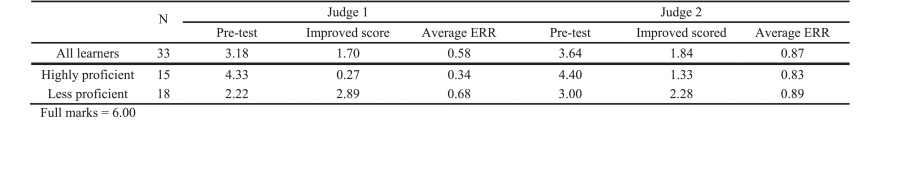
\includegraphics[height=3cm,width=15cm]{Table2.png}
%\counterwithin{figure}{section}
\centering
\caption{\textbf{Table 2.} Participant performance on pre-and post-tests}
\end{figure}

\begin{figure}[H]
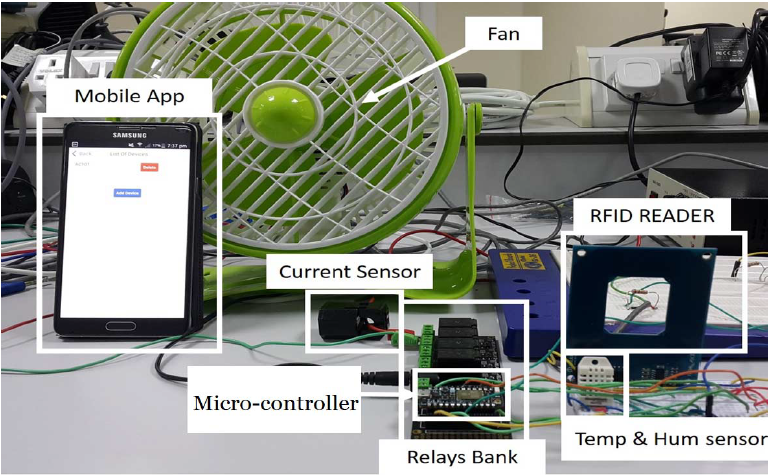
\includegraphics[height=8cm,width=16cm]{Figure3.png}
%\counterwithin{figure}{section}
\centering
\caption{\textbf{Figure 3.} Learning effectiveness of students with different proficiency levels}
\end{figure}

\paragraph{}
Next, we investigated whether RESOLVE was of great benefit to different learners (Table 2, second panel). To do so, the participants were divided into two groups based on their scores of the proficiency test, which was conducted in the first week. A total of 15 participants scored above or equal to the grand average (67.45), so they were classified as highly proficient. The other 18 participants with below-average scores were classified as less proficient. The average scores of the highly and less proficient groups were 80.93 and 56.22 out of 100.00 respectively. The learning effectiveness of the highly and less proficient students is visualized in Figure 3. Both figures showed that after the treatment, less proficient students made more noticeable improvement as compared with the highly proficient students. In fact, less proficient students achieved almost the same or even higher levels of performance in the emotion wording task than their counterparts. 
\paragraph{}
The significance of the improvements of both groups was further quantified by ANOVA: the first judge’s evaluation showed a significant difference between both the highly and less proficient learners (F(1, 31)=9.76, p value=0.004), whereas according to the second judge, no significant difference existed between the two groups (F(1, 31)=.71, p value=0.405). To understand whether less proficient learners benefited from the tool support, or highly proficient learners’ higher scores in the pre-test limited their potential for improvements, we calculated learner error reductions. Clearly, the ERRs of the less proficient learners were higher than those of the highly proficient learners based on both judges’ evaluations. It indicates that the less proficient learners made significant progress even after the error residual was normalized despite insignificant difference between the two groups in the second judge’s view. Since the results revealed that the less proficient learners showed greater improvements, we further sought to investigate how the performance of these two groups differed, which is discussed in the next section. 
\subsection{Performance Comparison of Learners}
\paragraph{}
The second research question attempted to explore how the improvements of highly and less proficient learners differed. A second order polynomial curve was used to fit these (proficiency level, improved score) data points: the trend is shown in Figure 4. From the first judge’s evaluation (left subfigure), a negative relationship can be seen between the learners’ language proficiency and their improved scores. In other words, the lower the proficiency level, the more improvement achieved by the participant. The second judge’s view, however, was somewhat different. The right figure reveals a downward trend for highly proficient learners and a slightly upward trend for less proficient learners. This means that for the highly proficient group, the higher the proficiency level, the smaller the gain; however, the less proficient learners did not follow this pattern. 
\paragraph{}
Taken together, the judges shared similar opinions with respect to the performance of the highly proficient learners whereas there were discrepancies for the less proficient learners. To investigate these differences, we scrutinized the individual performances of the less proficient participants. Discrepancies were found in four less proficient participants, so the data of these four participants were particularly examined. Table 3 shows the breakdown of the participants’ emotion words and their scores in the pre- and post-tests. 

\begin{figure}[H]
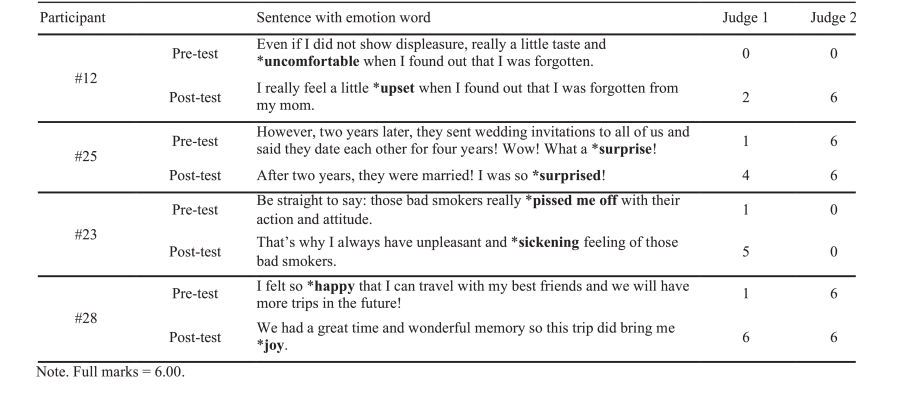
\includegraphics[height=7cm,width=16cm]{Table3.png}
%\counterwithin{figure}{section}
\centering
\caption{\textbf{Table 3.} Breakdown of four participants’ emotion word use and scores before and after treatment}
\end{figure}

\paragraph{}
Specifically, from the perspective of Judge 1, these four participants showed improvements whereas from Judge 2’s view, no one made progress except Participant 1. Although both judges agreed on Participant 1’s improvement, they were not consistent about the appropriateness of his emotion word use. We then take a further look at the performance of the other three participants from the evaluation of Judge 2. Participant 2 and Participant 4 received full marks in the pre- and post-tests, leaving no room for improvement. Turning to Participant 3, the zero point in both pre- and post-tests showed that his emotion words were the least appropriate. For this reason, the views of both judges differed greatly. Researchers such as Dewaele and Pavlenko suggest that the use of emotion words is related to individual experience; this could explain the judges’ divergent views. 
\paragraph{}
If we exclude the markedly different data, a similar trend can be seen in the judge evaluations as that seen in Figure 5. That is, for the less proficient group, the lower the proficiency level, the greater the improvement. In contrast, for highly proficient participants, the higher the proficiency level, the smaller their gains. This could be because they had confidence in their command of emotion words, as evidenced by the fact that seven out of 15 participants used the same emotion words in their pre- and post-writings, which scored full marks. On the other hand, 16 out of 18 participants used different emotion words in their writings. Their improved scores showed that their attempts were successful. 
\paragraph{}
It is worth noting that for the participants whose English proficiency was extremely high or extremely low, the bene- fit of RESOLVE was less obvious. It is not surprising that advanced learners had sufficient competence to make appropriate lexical choices. On the other hand, the low-achieving learners’ limited vocabulary was likely to make emotion word learning much more demanding. Overall, less proficient learners significantly benefitted from the proposed system, RESOLVE, in emotion word learning compared with the highly proficient learners, which was expected. 

\begin{figure}[H]
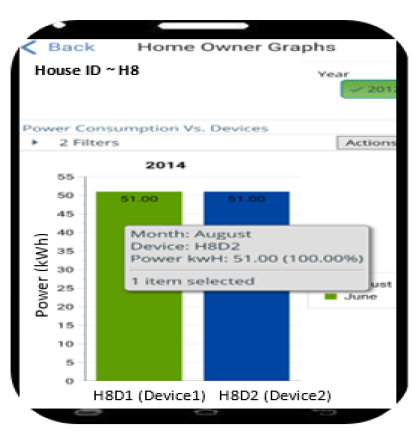
\includegraphics[height=7.5cm,width=16cm]{Figure4.png}
%\counterwithin{figure}{section}
\centering
\caption{\textbf{Figure 4.} Relationship between learner language proficiency and extent of improvement}
\end{figure}


\begin{figure}[H]
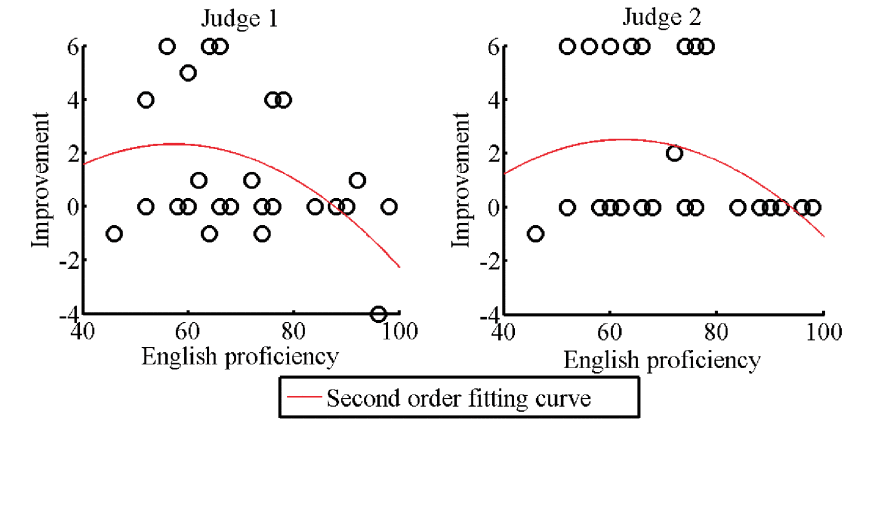
\includegraphics[height=7.5cm,width=16cm]{Figure5.png}
%\counterwithin{figure}{section}
\centering
\caption{\textbf{Figure 5.} Relationship between learner language proficiency and extent of improvement excluding the four outliers}
\end{figure}

\subsection{Learners’ Perceptions of Context-Based Emotion Synonym Learning}
\paragraph{}
To answer this research question, a seven-item reflection questionnaire was designed to elicit participant perceptions on RESOLVE in terms of learner needs, system usefulness, and its contribution to language learning. Moreover, participants’ open-ended responses were collected to elicit the rea- sons underlying their answers to each closed-form question. To have a greater understanding of the opinions of different students, the feedback of learners with different proficiency levels was analysed (Table 4). A two-sample t test was carried out, and the results showed no significant difference between the two groups’ responses. Learners’ perceptions on each survey question were discussed below. 
\paragraph{}
The first panel illustrates the participant learning back- grounds: their writing behaviour (item 1) and their needs for tool support (item 2). The scores of these two items were quite high (all above 3.80/5.00). Both groups reported that they intended to restate their feelings. To have a better under- standing of the behaviour of the two groups, we scrutinized the emotion words produced by the participants and found that eight highly and 16 less proficient participants used different emotion words in their pre- and post-writings. It is likely that highly proficient participants had greater confidence in their emotion word use than the less proficient ones. Meanwhile, participants’ strong demand for tool support indicated that learners needed help to be engaged in emotion word learning. 
\paragraph{}
The second panel shows participant perceptions on system usefulness, including system function (item 3) and suggested information (item 4-6). First, the tool usability scored quite high. In particular, both groups were satisfied with being able to consult synonyms and usage information directly without switching visual focus between webpages while composing their writing. The results supported previous research on the split-attention effect: Learning in an integrated environment reduces mental effort and improves learning results. Participants’ feedback showed that our design met their needs. Second, the information provided by RESOLVE included the ranked emotion words (item 4), the number of synonymous emotion words (item 5), and the usage information (item 6). Both groups appreciated the suggested emotion words as well as the usage information. Less proficient learners particularly acknowledged that the usage information (i.e., scenario descriptions, definitions and example sentences), benefit them in learning to use emotion synonyms appropriate to their contexts. Interestingly, both groups did not seem to share similar views on the number of suggested synonyms, even though there was no significant difference between them. Less proficient learners appreciated five suggestions whereas highly proficient participants expected more suggestions. Some participants suggested that eight synonyms would yield adequate choices for better wording. 
\paragraph{}
The last question (item 7) sought participant reflections on the role of RESOLVE for language proficiency. Nearly 80\% of the learners (26 out of 33 participants) saw RESOLVE as a practical reference aid that benefited their writing and promoted language competence. A significantly higher number of less proficient learners (n=16) acknowledged the tool assistance. The opinions of the less proficient participants echoed the findings of the previous research questions that they received greater benefit from the tool support than their counterparts. 

\begin{figure}[H]
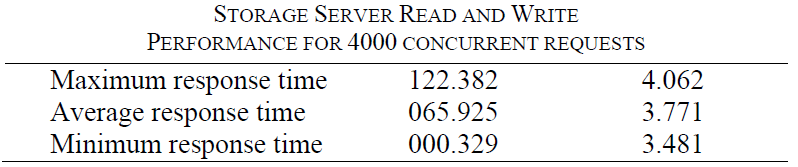
\includegraphics[height=5.9cm,width=15.4cm]{Table4.png}
%\counterwithin{figure}{section}
\centering
\caption{\textbf{Table 4.} Survey results of participant perceptions on RESOLVE}
\end{figure}

\newpage
\section{LIMITATIONS AND FUTURE WORK}
To the best of our knowledge, this is the first study considering the application of sentiment analysis to assisting language learning. It is worth mentioning that although the focus of the current study is emotion vocabulary learning, the RESOLVE system can be easily adapted for other vocabulary or synonym learning. While the preliminary findings supported that the developed system was beneficial to emotion word use, there are limitations in this study that could be improved. For example, a greater number of participants should be involved, which could help us take a closer look at potential learner difficulties in the use of emotion words. Also, tool comparison (e.g., online thesauri) could be conducted to examine their individual impacts on learners. 

\newpage
\section{CONCLUSION}
\paragraph{}
Emotion vocabulary has been an important concern in several disciplines. They were especially widely used in sentiment detection or prediction. However, it has not received particular attention in foreign language teaching and learning. In view of the paucity of research, we developed RESOLVE, a context-based emotion synonym suggestion system. Developed using machine learning techniques, RESOLVE is capable of suggesting contextually appropriate emotion synonyms. The usage information is also provided to reinforce learner’s word use. The tool effective- ness was assessed using a writing task and a reflection questionnaire. The results demonstrated that both the suggested emotion synonyms and the corresponding usage information are beneficial to learners’ use of emotion vocabulary. Notably, less proficient participants showed greater improvements.
\paragraph{}
Mastering emotion words is a challenging task for language learners, so emotion vocabulary should be explicitly taught and consciously learned. The RESOLVE system is applicable for use in classroom teaching and activities. The approach proposed in this study could be replicated in the classroom. Instructors could create various scenarios for specific emotion categories and have their students compose writings via consulting RESOLVE. Afterwards, instructors elaborate on how the words students produce could be used in various scenarios. Such pedagogical activities enable learners to develop a clearer understanding of as well as stronger command of emotion word use. 

\newpage
% \cleardoublepage
% \addcontentsline{toc}{section}{\textbf{References}}
% \addcontentsline{}{section}{\textbf{References}}

\section{REFERENCES}
\begin{thebibliography}{9}


\bibitem{d} J. Altarriba, ‘‘Emotion, memory, and bilingualism,’’ in \emph{Foundations of Bilingual Memory, }J. Altarriba and R. Heredia, Eds. New York, NY, USA: Springer, 2014, pp. 185–203.
\bibitem{d} A. Pavlenko, ‘‘Affective processing in bilingual speakers: Disembodied cognition?’’ \emph{ “Int. J. Psychol., }vol. 47, no. 6, pp. 405–428, 2012.
\bibitem{d} G. L. Clore and A. Ortony, ‘‘The semantics of the affective lexicon,’’ in \emph{Cognitive Perspectives on Emotion and Motivation. }New York, NY, USA: Springer, 1988, pp. 367–397.
\bibitem{d} E. H. Hovy, ‘‘What are sentiment, affect, and emotion? Applying the methodology of Michael Zock to sentiment analysis,’’ in \emph{Language Production, Cognition, and the Lexicon, }N. Gala, R. Rapp, and G. Bel-Enguix, Eds. Cham, Switzerland: Springer, 2015, pp. 13–24.
\bibitem{d} A.PavlenkoandV.Driagina,‘‘RussianemotionvocabularyinAmerican learners’ narratives,’’ \emph{Modern Lang. J., }vol. 91, no. 2, pp. 213–234, 2007.
\bibitem{d} C.-C. Huang and L.-W. Ku, ‘‘Interest analysis using semantic PageRank and social interaction content,’’ in \emph{Proc. IEEE 13th Int. Conf. Data Mining Workshops, }Dec. 2013, pp. 929–936.
\bibitem{d} P.-Y.Lu,Y.-Y.Chang,andS.-K.Hsieh,‘‘Causingemotionincollocation: An exploratory data analysis,’’ in \emph{Proc. 25th Conf. Comput. Linguistics Speech Process.,} 2013, pp. 236–249.
\bibitem{d} B.Pang,L.Lee,andS.Vaithyanathan,‘‘Thumbsup?:Sentiment classification using machine learning techniques,’’ in \emph{Proc. ACL Conf. Empirical Methods Natural Lang. Process.,} 2002, pp. 79–86.
\bibitem{d} J.-M. Dewaele, ‘‘Investigating the psychological and emotional dimensions in instructed language learning: Obstacles and possibilities,’’ \emph{Modern Lang. J.,} vol. 89, no. 3, pp. 367–380, 2005.
\bibitem{d} J.-M.Dewaele and A.Pavlenko,‘‘Emotionvocabularyininterlanguage,’’ \emph{Lang. Learn.,} vol. 52, no. 2, pp. 263–322, 2002.
\bibitem{d} T.Kaneko,‘‘Hownon-nativespeakersexpressanger,surprise,anxiety and grief: A corpus-based comparative study,’’ in \emph{Proc. Corpus Linguistics Conf.,} 2003, pp. 384–393.
\bibitem{d} E. M. Rintell, ‘‘That’s incredible: Stories of emotion told by second language learners and native speakers,’’ \emph{Developing Communicative Competence in a Second Language.} 1990, pp. 75–94.
\bibitem{d} J.-M. Dewaele, ‘‘On emotions in foreign language learning and use,’’ \emph{Lang. Teacher,} vol. 39, no. 3, pp. 13–15, 2015.
\bibitem{d} C. R. Graham, A. W. Hamblin, and S. Feldstein, ‘‘Recognition of emotion in English voices by speakers of Japanese, Spanish and English,’’ \emph{Int. Rev. Appl. Linguistics Lang. Teach.,} vol. 39, no. 1, pp. 19–37, 2001.
\bibitem{d} Y. Yeh, H.-C. Liou, and Y.-H. Li, ‘‘Online synonym materials and concor- dancing for EFL college writing,’’ \emph{Comput. Assist. Lang. Learn.,} vol. 20, no. 2, pp. 131–152, 2007.
\bibitem{d} M. Martin, ‘‘Advanced vocabulary teaching: The problem of synonyms,’’ \emph{Modern Lang. J.,} vol. 68, no. 2, pp. 130–137, 1984.
\bibitem{d} D. Liu, ‘‘Salience and construal in the use of synonymy: A study of two sets of near-synonymous nouns,’’ \emph{Cognit. Linguistics,} vol. 24, no. 1, pp. 67–113, 2013.
\bibitem{d} D. Liu and S. Zhong, ‘‘L2 vs. L1 use of synonymy: An empirical study of synonym use/acquisition,’’ \emph{Appl. Linguistics,} vol. 37, no. 2, pp. 239–261, Apr. 2016.
\bibitem{d} W.-F. Chen, M.-H. Chen, and L.-W. Ku, ‘‘Embarrassed or awkward? Ranking emotion synonyms for ESL learners’ appropriate wording,’’ in \emph{Proc. 10th Workshop Innov. NLP Building Educ. Appl.,} 2015, pp. 144–153.
\bibitem{d} W.-F. Chen, M.-H. Chen, M.-L. Chen, and L.-W. Ku, ‘‘A computer- assistance learning system for emotional wording,’’ \emph{IEEE Trans. Knowl. Data Eng.,} vol. 28, no. 5, pp. 1093–1104, May 2016.
\end{thebibliography}
\end{document}